% \documentclass[12pt, addpoints, answers]{exam}
\documentclass[12pt, addpoints]{exam}

\usepackage{amsmath, amssymb}
\usepackage{xcolor}
\usepackage{tikz}
\usepackage{enumerate}
\usepackage{graphicx}
\usepackage{tabularx}
\usepackage{algorithm}
\usepackage{algpseudocode}

\usepackage{graphics}
\usepackage{tikz}
\usepackage{tikz-qtree}
\usepackage{drawstack}

\usetikzlibrary{graphs}
\tikzset{every tree node/.style={minimum width=2em,draw,circle},
    blank/.style={draw=none},
    edge from parent/.style=
    {draw,edge from parent path={(\tikzparentnode) -- (\tikzchildnode)}},
    level distance=1.2cm}

\newcommand{\red}[1]{\textcolor{red}{#1}}
\newcommand{\blue}[1]{\textcolor{blue}{#1}}

% For inserting code snippets.
\usepackage{listings}
\lstset{
    columns = fixed,
    basewidth = {0.5em},
    breaklines = true,
    backgroundcolor = \color{white},
    keywordstyle = \color[RGB]{40, 40, 255},
    numberstyle = \footnotesize\color{darkgray},
    commentstyle = \ttfamily\color{violet},
    basicstyle = \ttfamily,
    stringstyle = \ttfamily\color[RGB]{128, 0, 0},
    showstringspaces = false,
    language = {[11]C++},
    escapechar = \@
}
\lstnewenvironment{cpp}[1][]{\lstset{language = {[11]C++}, #1}}{}

\renewcommand{\baselinestretch}{1.15}
\setlength{\parskip}{1.25\baselineskip}

% headers, footers, titles
\title{CS101A(H) Homework 6}
\author{}
\date{Due date: December 2, 2025, at 20:00}

% formats of questions, choices, points, etc.
\qformat{\bf\thequestion. (\totalpoints\ points) \thequestiontitle\hfill}
\pointname{'}
\CorrectChoiceEmphasis{\bf\color{blue}}
\SolutionEmphasis{\color{blue}}

% We frequently use this font.
\newcommand{\ttt}{\texttt}
\newcommand{\bluett}[1]{\textcolor{blue}{\ttt{#1}}}

\begin{document}

\maketitle

Your grade for this homework will be computed as
\[
\min\bigl(\text{Single Choices}+\text{Multiple Choices} + \text{Others},\; 50 \text{ pts}\bigr) .
\]

\textbf{Notes: } \textbf{Unless otherwise stated, always express your final asymptotic bounds using} \(\boldsymbol{\Theta(\cdot)}\) \textbf{notation for tight complexity, not just} \(O(\cdot)\) \textbf{or} \(\Omega(\cdot)\).  
All answers must be written \textbf{inside the provided answer boxes} and \textbf{in English}. When submitting, match your solutions to the problems correctly in Gradescope. No late submission will be accepted. Failure to follow these rule may result in partial or full loss of credit.



\paragraph{Usage of AI.}
The use of AI tools for searching information or obtaining assistance on this homework is strictly prohibited. All solutions must be derived from your own understanding and effort. Submissions will be reviewed carefully, and any indication of reliance on AI-generated content will result in severe penalties.

\paragraph{Academic Integrity.}
This course upholds the highest standards of academic integrity. Any form of academic dishonesty, including plagiarism, unauthorized collaboration, or the use of prohibited resources such as AI tools, will be treated as a serious violation. Such actions not only undermine your own learning but also violate university policies. 

\begin{questions}

\newpage
\titledquestion{Single Choice}

\begin{parts}

\part[2] Choose the \textit{incorrect} statement about tree.
\begin{choices}
  \choice Nodes with the same parent are siblings
  \choice Leaf nodes always have a degree equal to 0.
  \choice A tree of depth 2 has a maximum of 7 nodes.
  \choice Each node, other than the root, has exactly one node pointing to it.
\end{choices}

\part[2] Choose the correct statement.
\begin{choices}
  \choice We can use a stack to get the breadth-first traversal result of a tree.
  \choice The BFS result of the figure below is ABHCDIGEFJK.
\begin{figure}[H]
    \centering
    \includegraphics[width=0.35\linewidth]{imgs/q1-2.png}
\end{figure}

  \choice The memory required by DFS is  $\Theta(n)$.
  \choice The time complexity of BFS and DFS are both $\Theta(n)$.
\end{choices}


\part[2] Which traversals of the left tree and right tree, will produce the same sequence node name?

\begin{minipage}{1\textwidth}
\centering
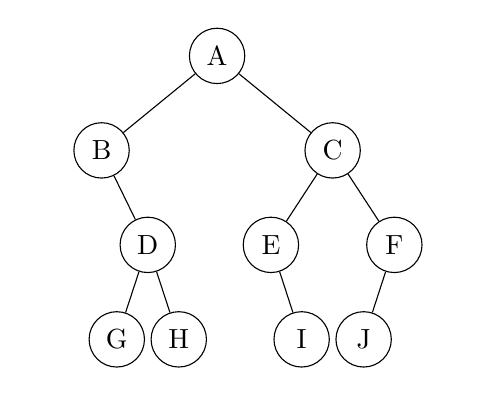
\begin{tikzpicture}
\Tree
[.A
[.B
        \edge[blank]; \node[blank]{};
        \edge[];[.D
            \edge[];[.G
            ]
            \edge[]; [.H
            ]
        ]
    ]
    [.C
        \edge[];[.E
            \edge[blank]; \node[blank]{};
            \edge[];[.I
            ]
        ]
        \edge[];[.F
             \edge[];[.J            ]
             \edge[blank]; \node[blank]{};
            ]
        ]
    ]
\end{tikzpicture}
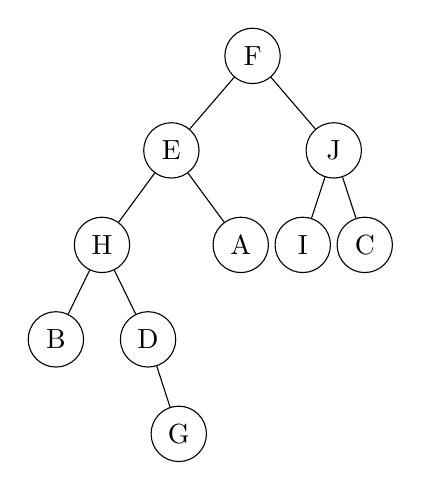
\begin{tikzpicture}
\Tree
[.F
    [.E
            \edge[];[.H
                \edge[];[.B ]
                \edge[];[.D
                \edge[blank]; \node[blank]{};
                    \edge[];[.G 
                        ] 
                    ]
            ]
            \edge[]; [.A
            ]
        ]
        [.J
        \edge[];[.I
        ]
        \edge[];[.C
        ]
        ]
    ]
\end{tikzpicture}
\end{minipage} \\

\begin{choices}
  \choice  left: Post-order, right: Pre-order 
  \choice  left: In-order, right: Pre-order 
  \choice  left: Post-order, right: In-order
  \choice  left: In-order, right: Post-order 
\end{choices}

\part[2] Choose the \textit{incorrect} statement about Huffman coding.
\begin{choices}
  \choice Huffman coding prioritize characters based on their frequencies in text.
  \choice If character $a$ has a higher frequency than $b$, then the encoded $a$ has a length no longer than encoded $b$.
  \choice No code is a prefix of another code.
  \choice Given the set of characters and the \textbf{order} of their frequencies but the exact frequencies unknown, we can still determine the length of each encoded character.
\end{choices}


\part[2] Choose the correct statement about binary search tree.
\begin{choices}
  \choice Almost all of the relevant operations on a binary search tree are $O(h)$, where $h$ is the height of the tree.
  \choice When deleting a node with two children, we first replace it with the smallest node on the right sub-tree or the smallest node on the left sub-tree.
  \choice Given an array, suppose we construct a BST (without balancing) by sequentially inserting the elements of the array into an empty BST. Then the time complexity of this process is $O(n \log n)$ in all cases.
  \choice The in-fix order traversal of a BST is an array of descending order.
\end{choices}


\end{parts}

\newpage
\titledquestion{Multiple Choices}

Each question has \textbf{one or more} correct answer(s). Select all the correct answer(s). For each question, you will get 0 points if you select one or more wrong answers, but you will get half points if you select a non-empty subset of the correct answers.

\begin{parts}

\part[3] Choose the correct statement(s) about tree.
\begin{choices}
  \choice The length of a path is number of nodes in the path.
  \choice There is only one root in a tree.
  \choice The degree of a node is positive.
  \choice For every node in the tree, there is one parent node.
  \choice The height of a binary tree is always positive.
\end{choices}

\part[3] Choose the correct statement(s) about binary tree whose height is $h$, where $h$ greater than 3.
\begin{choices}
  \choice  Suppose it is a perfect binary tree with $l$ leaf nodes, then this tree has $l-1$ internal nodes.
  \choice  Suppose it is a complete tree whose left sub-tree has $n$ nodes, then the range of $n$ is between $2^{h-1}+1 $ and $2^h$.
  \choice  Suppose it is a full binary tree, the number of nodes is always no less than $2^{h}$.
  \choice If the result of in-order traversal of an expression tree is $3\times 4 \times 5 + 1 + 2 + 5 \div 5 + 6 - 7 $, then the result of the expression represented by this tree can be 63.
\end{choices}


\part[3] Choose the correct statement about heap using complete trees.
\begin{choices}
  \choice In the worst case, the time complexity of \texttt{Push} operation is $\Theta(n)$ if we do not use complete tree to implement a heap.
  \choice  Usually \texttt{Push} operation takes $O(\log n)$ time.
  \choice  Heap sort with a max-heap takes $\Theta(n \log n)$ time and is an in-place sorting algorithm.
  \choice Merging two binary heaps of size n is a $\Theta(n)$ operation
\end{choices}


\part[3] Consider an AVL tree whose number of nodes is $n$ and height is $h$, which of the following are true?

\begin{choices}
  \choice Inserting or removing a node can increase the height of a tree by at most 1.
  \choice An insertion on a perfect binary tree (which is also an AVL tree) can cause an imbalance.
  \choice $h$ may equals to $\Theta(n)$ in worst case.
  \choice $n= O(2^h)$
\end{choices}

\part[3] Choose the correct statement about binary search tree.

\begin{choices}
  \choice In a BST, the nodes in a subtree appear contiguously in the in-order traversal sequence of the BST.
    \choice If we erase a node that has two children, then it can be replaced by the maximum object in its right subtree.
    \choice There are 5 different  BSTs of a set with 3 distinct numbers.
    \choice If a node doesn't have a right subtree, then its \textbf{next} (defined in lectures) object is the largest object (if any) that exists in the path from the node to the root.
\end{choices}

\end{parts}

\newpage
\include{run_dfs_and_bfs}

\newpage
\titledquestion{Draw a binary tree}
\begin{parts}
    \part[3]Given the in-order and pre-order traversal of a binary tree T are IGDHBAECF and ABDGIHCEF respectively.\\
    Draw the tree T.

    \vspace{7cm}

    \part[3]Given the in-order and post-order traversal of a binary tree T are ADHGKLMRUXTW and AHDLKGUXRWTM respectively.\\
    Draw the tree T.

    \vspace{7cm}

    \newpage
    \part[2] Given the pre-order and post-order traversal of a binary tree T, can you decide the tree T? If yes, please describe an algorithm to construct T; if no, please provide a counterexample.
    
    \vspace{7cm}
\end{parts}

\newpage
\include{Huffman}

\newpage
\titledquestion{AVL tree operations}

Here is an AVL tree. Denote it as $T$.

\begin{center}
    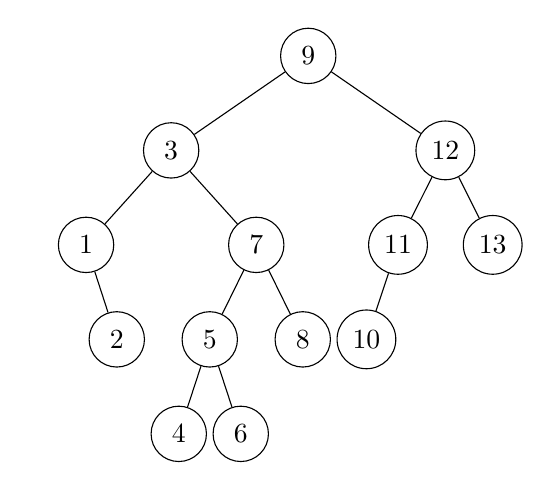
\begin{tikzpicture}[]
    \Tree
    [.9
        [.3
            [.1
                \edge[blank]; \node[blank]{};
                [.2
                ]
            ]
            [.7
                [.5
                    [.4
                    ]
                    [.6
                    ]
                ]
                [.8
                ]
            ]
        ]
        [.12
            [.11
                [.10
                ]
                \edge[blank]; \node[blank]{};
            ]
            [.13
            ]
        ]
    ]
    \end{tikzpicture}
\end{center}

\begin{parts}

\part[2] Insert $5.5$ into $T$. Draw the AVL tree before checking if any balance correction is needed.

\vspace{6cm}


\part[2] Insert $5.5$ into $T$. Draw the AVL tree after balance corrections.

\vspace{7cm}

\part[2] Remove $12$ from $T$ (\textbf{NOT from the previous answer!}). Draw the AVL tree after replacing and before checking if any balance correction is needed.

\textbf{Note}: when erasing a non-leaf node $x$, we will follow the way in BST lecture slides to replace $x$ with
\begin{itemize}
    \item the child of $x$, if $x$ has exactly one child, or
    \item the successor of $x$, if $x$  has two children
\end{itemize}

\vspace{6cm}

\part[2] Remove $12$ from $T$. Draw the AVL tree after balance corrections.

\vspace{6cm}

\end{parts}

\end{questions}

\end{document}